\chapter{Despliegue y resultados}\label{CAP:Despliegueyresultados}
A lo largo del desarrollo del proyecto, todo el trabajo ha ca\'ido sobre mi, pero llegados a este punto los aut\'enticos protagonistas son los usuarios, los alumnos de la ETSIT, tanto los que han disfrutado de un programa erasmus como los que no. Y aqu\'i es donde su opini\'on cuenta, ya que ser\'an ellos quienes hagan uso de la aplicaci\'on. Este pen\'ultimo apartado lo dedicaremos a la explicaci\'on de los distintos pasos llevados a cabo para realizar debidamente el despliegue y las pruebas de la aplicaci\'on web.\\
 
\section{Despliegue de la aplicaci\'on}
Para llegar al funcionamiento deseado de la aplicaci\'on se han realizado diversas pruebas tanto internas como externas y con una dimensi�n mayor de usuarios. Para las pruebas externas se han realizado de distinta manera.\\

\subsection{Primera prueba: Servidor local}
A la vez que se va implementando todo el c\'odigo de la aplicaci\'on, se van ejecutando una serie de pruebas, para ir depurando peque�os bloques de funcionalidades. Estas pruebas se realizan lanzando un servidor local con el que podemos simular una navegaci�n por internet. El navegador lanzar� peticiones HTTP al servidor, el cu\'al ir\'a mostr\'andole la informaci\'�n que el cliente le pida.\\

En primer lugar, para poder observar correr una p\'agina Django con el servidor de pruebas sin la necesidad de lenvantar un servidor \textit{Apache} y configurarlo con python... basta con ejecutar la siguiente l\'inea en una \textbf{shell Unix} \textit{manage.py runserver}. Si no se le indica ninguna IP ni puerto al lanzar el servidor de python, dicho servidor se ata a la IP local (\textit{localhost} o 127.0.0.1) y a un puerto cualquiera, que por defecto python toma el puerto de escucha 8000.\\

\begin{figure}[htbp]
	
	\centering
	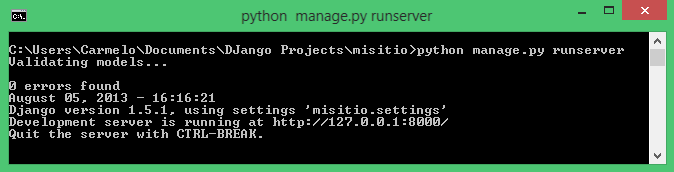
\includegraphics[scale=0.5]{./Figuras/despliegue/localhost.jpg}
	\caption{Servidor local Django.}
	\label{fig:svdlocaldjango}
	
\end{figure}

Con estas pruebas, servidor local, se ha depurado m\'as del 80\% del c\'odigo. Pudiendo avanzar con el desarrollo de la aplicaci\'on, y poder realizar las pautas necesarias para las siguientes pruebas del despliegue de la herramienta web.\\

\subsection{Segunda prueba: Servidor local con acceso a Internet}
Esta segunda prueba, que consideramos el primer despliegue con unas dimensiones mayores de la aplicaci\'on fue el momento clave para saber si a los usuarios les resultaba \'util o no algunos requisitos de la aplicaci\'on web.\\

En esta ocasi\'on se pretend\'ia lanzar el propio servidor que ven\'ia instalado con Django, pero abriendo un puerto a Internet, es decir, poder llegar a este servidor desde cualquier m\'aquina ajena a nuestra red dom\'stica. Para ello al lanzar el servidor de Django debemos indicarle el puerto y la IP en las que el servidor estar\'a escuchando. En una \textbf{shell Unix} ejecutamos \textit{manage.py runserver 192.168.1.129:8000}.\\

Para acceder a la aplicaci\'on desde un PC o un dispositivo conectado a la LAN de casa o a la WiFi de casa la url que hay que poner en el navegador es \textit{192.168.1.129:8000\tuerasmus}. En cambio, para acceder a la aplicaci\'on web desde un PC o dispositivo m\'ovil proveniente de Internet, totalmente ajeno a nuestra red de casa, la url ser\'a \textit{37.134.69.14:8000\tuerasmus}. Esta IP es la IP p\'ublica de nuestra conexi\'on Internet. Para abrir este puerto a Internet se contact\'o con la compa\~nia telef\'onica, indic\'andoles que abriesen dicho puerto al exterior.\\

El servidor se mantuvo lanzado unas dos semanas, y unos cuantos usuarios estuvieron probando la aplicaci\'on y notific\'andome de los bugs que iban obteniendo durante este periodo de pruebas. Adem\'as de reportarme los bugs que iban encontrando, fue bastante valioso el feedback acerca de la funcionalidad de la aplicaci\'on y de posibles mejores que se podr\'ian aplicar.\\

\subsection{Alojamiento web}
Como \'ultimo y definitivo m\'etodo de despliegue se hizo uso de hosting. Se eligi\'o la web de \textbf{Alwaysdata}, que permite el despliegue de aplicaciones web implementadas en Django (python), con lo que no hay que hacer ninguna instalaci\'on. El servidor que tiene integrado es un servidor Apache.\\

\begin{figure}[htbp]
	
	\centering
	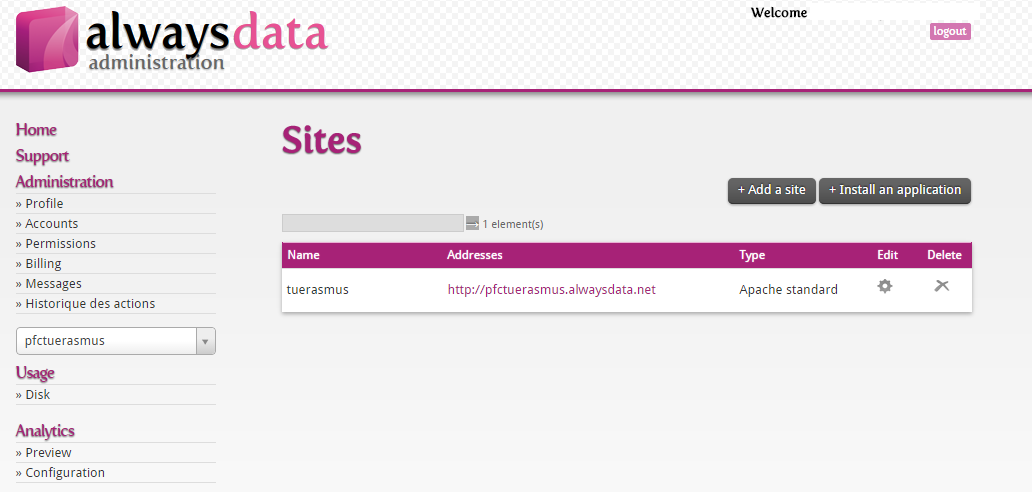
\includegraphics[scale=0.5]{./Figuras/despliegue/cuentaAlwaysdata.png}
	\caption{Cuenta para despliegue TuErasmus de Alwaysdata.}
	\label{fig:cuentaAlwaysdata}
	
\end{figure}

Para conseguir un despliegue exitoso, fue necesario conectar mediante conexi\'on ssh desde una \textit{shell Unix} a la cuenta con la que se realizar\'o el despliegue, ejecutando la siguiente l\'inea: \textit{ssh pfctuerasmus@ssh.alwaysdata.com}. De esta manera nos conectamos al directorio home de nuestra cuenta donde deberemos copiar mediante scp un fichero ".zip" que contenga nuestro proyecto completo django:  \textit{scp mypfc.zip pfctuerasmus@ssh.alwaysdata.com: \home\pfctuerasmus\mypfc}.\\

Una vez copiado el zip, debemos descomprimir y realizar unas modificaciones en el directorio que acabamos de copiar del proyecto django. Cuando tengamos descomprimido el fichero .zip, debemos navegar en nuestro proyecto y situarnos en el directorio ra\'iz del proyecto (directorio donde se encuentre el fichero \textit{manage.py}) y crearemos una carpeta llamada \textit{public}, en la que crearemos dos fichero: \textit{django.fcgi} y \textit{.htaccess} que nos permitir\'an mantener lanzada nuestra aplicaci\'on y poder acceder y navegar por ella en cualquier momento.\\

\begin{figure}[htbp]
	
	\centering
	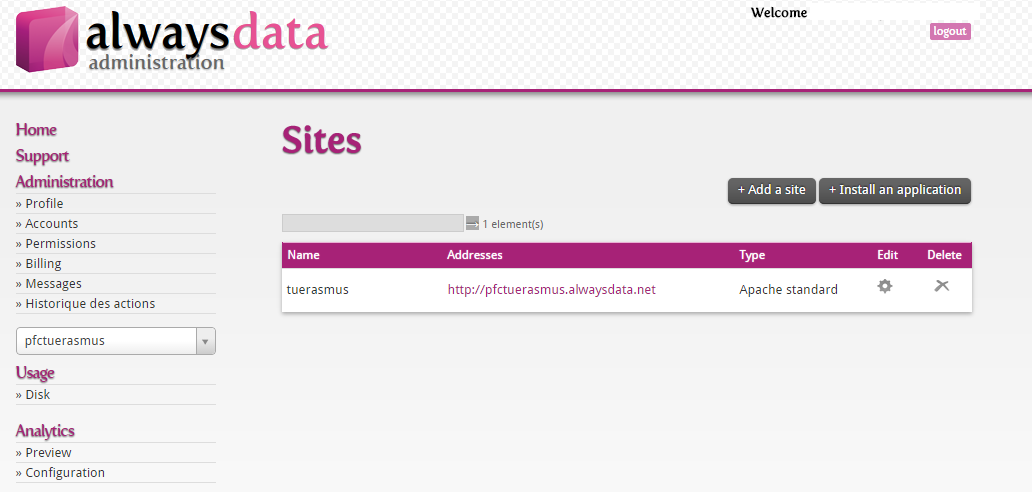
\includegraphics[scale=0.5]{./Figuras/despliegue/cuentaAlwaysdata.png}
	\caption{Directorio de la cuenta de Alwaysdata donde encontramos los ficheros y directorio que forman nuestro proyecto Django.}
	\label{fig:directorioSSH}
	
\end{figure}

Adem\'as de estos dos ficheros, debemos crear un enlace simb\'olico, para permitir el acceso del admin de Django desde la web de Alwaysdata, y que esta interfaz del admin coja los ficheros est\'aticos de estilo de donde corresponde.\\

Y con esto se complet\'o el ciclo de las configuraciones para conseguir que la aplicaci\'on est\'e corriendo debidametne desde el hosting.\\

\section{Resultados de las pruebas}
Una vez desplegada la aplicaci\'on, con el segundo m\'etodo (IP p\'ublica), la reacci\'on de los usuarios fue positiva, pero no tanto como se esper\'o. Por loq ue tuvimos que realizar una serie de mejoras para motivar el uso de la aplicaci\'on web y que los usuarios quedasen satisfechos con los resultados.\\

Con el segundo despliegue masivo (alojamiento web) la usabilidad de la aplicaci\'on qued\'o mucho m\'as clara y mejor definida. Con lo que los resultados de este segundo despliegue se acercan m\'as a lo deseado. Como todo periodo de pruebas siempre surgen bugs que se fueron mitigando a medida que fueron apareciendo.\\

Por tanto, quedamos satisfechos con los resultados obtenidos. Y tras estas pruebas, el feedback de los usuarios ha sido bastante constructivo ya que se han abierto de esta manera futuras l\'ineas para seguir trabajando en dicho proyecto.\\

\section{Problemas encontrados}
Como problemas encontrados en el despliegue de la aplicaci\'on, se ha de mencionar la ausencia de motivaci\'on que ofrec\'ia la aplicaci\'on. Por lo que no se consigui\'o una total satisfacci\'on en cuanto a las pruebas que se deseaban desde un principio.\\

Uno de los bugs que primero surgieron con el segundo m\'etodo de despliegue (hosting) fueron los ficheros est\'aticos de la aplicaci\'on. El path de cada fichero de estilo no era el correcto y por tanto cuando acced\'ias a las p\'aginas de la aplicaci\'on estas eran mostradas con un aspecto nada similar a lo dise\~nado.\\

Una mejora realizada, resultante de este m\'etodo de despliegue, fue aprovechar el cacheo de los ficheros de Javascript (jquery.js) usados en el c\'odigo donde se integraban los mapas de \textit{Google Maps} para la locaclizaci\'on de las universidades y de las residencias. Esto mejorar\'ia el rendimiento de la aplicaci\'on web, ya que se evit\'o tener estos ficheros en local y se ped\'ian directametne desde Internet, con lo que si est\'an con anterioridad cacheados ahorramos tiempo y espacio.\\

Adem\'as de estos dos problemas mencionados en las l\'ineas superiores, se tuvo que solucioanr otro problema relacionado con la configuraci\'on de la aplicaci\'on, ya que constantemente aparec\'ia el mensaje de error "500: \textit{Internal Server Error}", cuya raz\'on era la configuraci\'on err\'onea de la cuenta creada para el despliegue en alwaysdata.\\

